% !Rnw root = learnR.Rnw

%% ---preamble.tex----%% 
%% maxwidth is the original width if it is less than linewidth
%% otherwise use linewidth (to make sure the graphics do not exceed the margin)
\makeatletter
\def\maxwidth{ %
  \ifdim\Gin@nat@width>\linewidth
    \linewidth
  \else
    \Gin@nat@width
  \fi
}
\makeatother

\definecolor{fgcolor}{rgb}{0.345, 0.345, 0.345}

\definecolor{shadecolor}{rgb}{.97, .97, .97}
\definecolor{messagecolor}{rgb}{0, 0, 0}
\definecolor{warningcolor}{rgb}{1, 0, 1}
\definecolor{errorcolor}{rgb}{1, 0, 0}






This chapter is a tour through models and methods that are
straightforward to fit using R.  Some of these lend themselves
to relatively automated use.   There is some limited attention
to the traps that can catch users who are unwary, or who have
ventured too easily into areas that call for some greater level
of statistical sophistication than their training and experience
has given them.

In each case, comments with be introductory and brief.  Firstly, there
are brief comments on the fitting of smooth curves.  The first and
second topics highlight specific types of departure from the iid
(independently and identically distributed) assumption.

\section{Hierarchical Multilevel Models}\label{sec:hmlm}

\noindent
\fbox{
\parbox{\textwidth}{{\bf Models with Non-iid Errors -- Multilevel models}:\\[4pt]
\begin{tabular}{ll}
Error Term & Errors do not have to be (and often are not) iid\\[6pt]
Multilevel & Multilevel models are a (relatively) simple type of
\\ models & non-iid model, implemented using \code{lme()}
(\pkg{nlme}) or \\ & \code{lmer()}\ (\pkg{lme4} package).\\ & Such
models allow different errors of prediction,\\ & depending on the
intended prediction.
\end{tabular}
}}
\begin{marginfigure}
\begin{Schunk}


\centerline{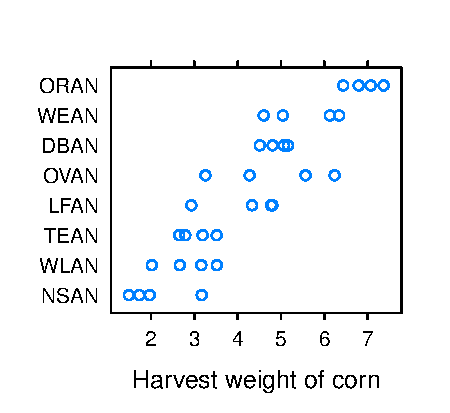
\includegraphics[width=0.98\textwidth]{figs/9-ant111b-1} }

\end{Schunk}
\caption{Yields from 4 packages of land on each of eight sites on the
  Caribbean island of Antigua. Data are a summarized version of a
  subset of data given in Andrews and Herzberg 1985,
  pp.\~339-353.\label{fig:caribbean}}
\end{marginfigure}
\vspace*{15pt}

Figure \ref{fig:caribbean} shows corn yield data from the Caribbean island of
Antigua, as in the second column (`Yields') of Table \ref{tab:ant111b}.
Each value is for one package of land.
The code for the figure is:
\begin{Schunk}
\begin{Sinput}
ant111b <- DAAG::ant111b
Site <- with(ant111b, reorder(site, harvwt,
                              FUN=mean))
lattice::stripplot(Site ~ harvwt, data=ant111b,
          scales=list(tck=0.5),
          xlab="Harvest weight of corn")
\end{Sinput}
\end{Schunk}

\begin{table}
\begin{center}
{\small
\begin{tabular}{@{}rc||r@{\hspace{1mm}}lcc@{}}
\hline
\multicolumn{1}{c}{Location}  & \multicolumn{1}{c}{Yields}  &
\multicolumn{2}{l}{Location} & Residuals from\\
 & & \multicolumn{2}{l}{effect} & \multicolumn{1}{c}{location mean}\\
\hline
DBAN &  5.16, 4.8, 5.07, 4.51 &  \vline& $+$0.59 & 0.28, $-$0.08, 0.18, $-$0.38 \\
LFAN &  2.93, 4.77, 4.33, 4.8 &  \vline& $-$0.08 &  $-$1.28, 0.56, 0.12, 0.59 \\
NSAN & 1.73, 3.17, 1.49, 1.97 &  \vline& $-$2.2 & $-$0.36, 1.08, $-$0.6, $-$0.12 \\
ORAN & 6.79, 7.37, 6.44, 7.07 & $_{(4.29)} $ \vline& $+$2.62 & $-$0.13, 0.45, $-$0.48, 0.15 \\
OVAN & 3.25, 4.28, 5.56, 6.24 &  \vline& $+$0.54 &  $-$1.58, $-$0.56, 0.73, 1.4 \\
TEAN & 2.65, 3.19, 2.79, 3.51 &  \vline& $-$1.26 & $-$0.39, 0.15, $-$0.25, 0.48 \\
WEAN &  5.04, 4.6, 6.34, 6.12 &  \vline& $+$1.23 &  $-$0.49, $-$0.93, 0.81, 0.6 \\
WLAN & 2.02, 2.66, 3.16, 3.52 &  \vline& $-$1.45 & $-$0.82, $-$0.18, 0.32, 0.68 \\
\hline
\end{tabular}
}
\caption{The leftmost column has harvest weights (\code{harvwt}), for
  the packages of land in each location, for the Antiguan corn data.  Each of
  these harvest weights can be expressed as the sum of the overall
  mean (= 4.29), location effect (third column), and residual from the
  location effect (final column).
\label{tab:ant111b}}
\end{center}
\vspace*{-0pt}
\end{table}
\vspace*{3pt}

Depending on the use that will be made of the results, it may be
essential to correctly model the structure of the random part of the
model.  In comparing yields from different packages of land, there are
two sorts of comparison.  Packages on the same location should be
relatively similar, while packages on different locations should be
relatively more different, as Figure \ref{fig:caribbean} suggests.
A prediction for a new package at one of the existing locations is
likely to be more accurate than a prediction for a totally new
location.

\marginnote[10pt]{Because of the balance the corn yield data, an
analysis of variance that specifies a formal \code{Error} term is
an alternative to the fitting of a multilevel model.}  Multilevel
models are able to account for such differences in predictive
accuracy.  For the Antiguan corn yield data, it is necessary to
account both for variation within sites and for variation between
sites.  The R packages \pkg{nlme} and \pkg{lme4} are both able to
handle such data.

\section{Regular Time Series in R}\label{sec:ts}
\noindent
\fbox{
\parbox{\textwidth}{{\bf Models with Non-iid Errors -- Time Series}:\\[4pt]
\begin{tabular}{ll}
Time & Points that are close together in time commonly show\\
sequential & a (usually, +ve) correlation. R's \code{acf()} and
\code{arima()}\\ & functions are powerful tools for use with time
series.
\end{tabular}
}}
\vspace*{15pt}

Any process that evolves in time is likely to have a
sequential correlation structure.  The value at the current
time is likely to be correlated with the value at the previous
time, and perhaps with values several time points back.
The discussion that follows will explore implications for data
analysis.

\subsection{Example -- the Lake Erie data}



\begin{figure}
\begin{Schunk}


\centerline{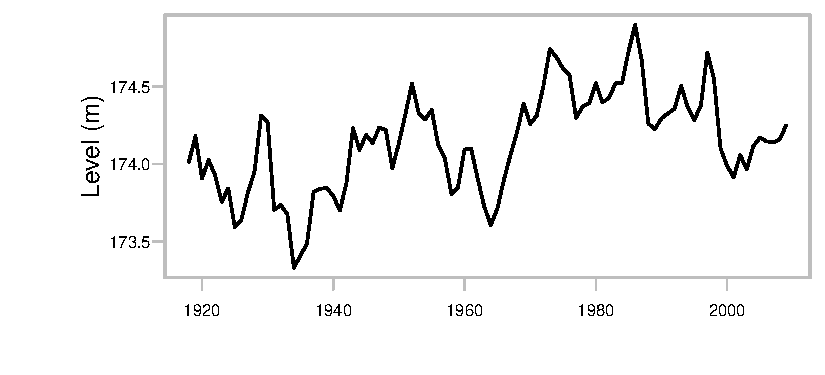
\includegraphics[width=0.98\textwidth]{figs/9-Erie1-1} }

\end{Schunk}
\caption{Lake Erie levels (m).
}\label{fig:erie}
% \setfloatalignment{t}
\end{figure}
\begin{marginfigure}[-7cm]
\begin{Schunk}
\begin{Sinput}
Erie <- DAAG::greatLakes[,"Erie"]
plot(Erie, xlab="", fg="gray",
     ylab="Level (m)")
\end{Sinput}
\end{Schunk}
\end{marginfigure}

The data series \code{Erie}, giving levels of Lake Erie
from 1918 to 2009, will be used as an example from which
to start the discussion.\sidenote{Data are
  from {\scriptsize
\url{http://www.lre.usace.army.mil/greatlakes/hh/greatlakeswaterlevels/historicdata/greatlakeshydrographs/}}}
    The series is available as the column \code{Erie} in the
    multivariate time series object \code{DAAG::greatLakes}.

Figure \ref{fig:erie} shows a plot of the series.

\begin{figure}
\begin{Schunk}


\centerline{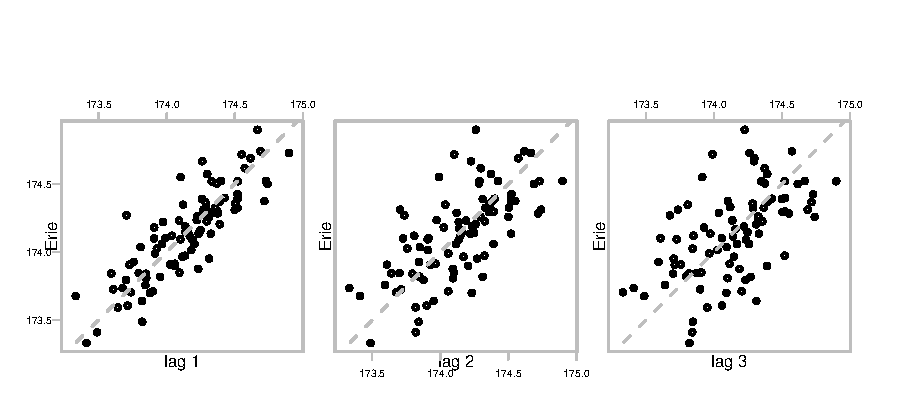
\includegraphics[width=0.98\textwidth]{figs/9-lagErie-1} }

\end{Schunk}
\vspace*{-3pt}

\begin{Schunk}


\centerline{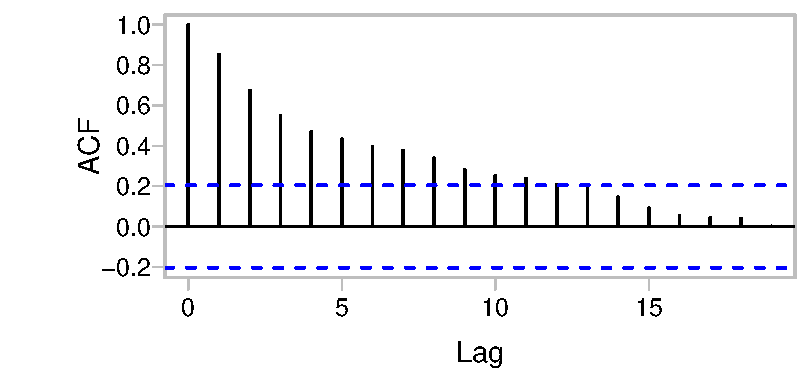
\includegraphics[width=0.7\textwidth]{figs/9-acfErie-1} }

\end{Schunk}
\caption{Panel A plots Lake Erie levels vs levels at lags 1, 2 and 3
  respectively. Panel B shows a consistent pattern of decreasing
  autocorrelation at successive lags.
}\label{erie-lagplot}
\vspace*{-6pt}
\end{figure}

\begin{marginfigure}[-10cm]
\begin{Schunk}
\begin{Sinput}
## Panel A
lag.plot(Erie, lags=3,
         do.lines=FALSE,
         layout=c(1,3), fg="gray",
\end{Sinput}
\end{Schunk}
\begin{Schunk}
\begin{Sinput}
## Panel B
acf(Erie, main="", fg="gray")
\end{Sinput}
\end{Schunk}
\end{marginfigure}

\marginnote{Where values of covariates are available that largely
or partly explain the dependence, it may make sense to account for
these in the model. The details of how this should be done will
depend on the intended use of the model.}

The plots in Figure \ref{erie-lagplot} are a good starting point for
investigation of the correlation structure.  Panel A shows lag plots,
up to a lag of 3.  Panel B shows estimates of the successive
correlations, in this context are called autocorrelations.

There is a strong correlation at lag 1, a strong but weaker
correlation at lag 2, and a noticeable correlation at lag 3.  Such
a correlation pattern is typical of an autoregressive process where
most of the sequential dependence can be explained as a flow-on
effect from a dependence at lag 1.

In an autoregressive time series, an\marginnote{An autoregressive
  model is a special case of an Autoregressive Moving Average (ARMA)
  model.}  independent error component, or \textit{innovation} is
associated with each time point. For an order $p$ autoregressive time
series, the error for any time point is obtained by taking the
innovation for that time point, and adding a linear combination of the
innovations at the $p$ previous time points.  (For the present time
series, initial indications are that $p=1$ might capture most of the
correlation structure.)

\subsection{Patterns that are repeatable}

Smoothing terms can be fitted to the pattern apparent in
  serially correlated data, leaving {\em errors} that are pretty much
  uncorrelated.  Such a pattern is in general, however, unrepeatable.
  It gives little clue of what may happen the future.  A re-run of
  the process (a new {\em realization}) will produce a different
  series, albeit one that shows the same general tendency to move up
  and down.

What sorts of patterns may then be repeatable?  Indications that a
pattern may be repeatable include:
\begin{itemize}
\item A straight line trend is a good starting point for some
  limited extrapolation. But think: Is it plausible that the trend
  will continue more than a short distance into the future?
\item There may be a clear pattern of seasonal change, e.g.,
with seasons of the year or (as happens with airborne pollution)
with days of the week. If yearly seasonal changes persist over
different years, or weekly day-of-the-week changes persist over
different weeks, these effects can perhaps be extrapolated with
some reasonable confidence.
\item There is a regression relationship that seems likely to
explain future as well as current data.
\end{itemize}

An ideal would be to find a covariate or covariates than can largely
explain the year to year changes.  For this series, this does not seem
a possibility.  In the absence of identifiable direct cause for the
year to year changes, a reasonable recourse is to look for a
correlation structure that largely accounts for the pattern of the
year to year change.  

\subsection*{Smooth, with automatic choice of smoothing parameter}

\begin{figure}
\begin{Schunk}


\centerline{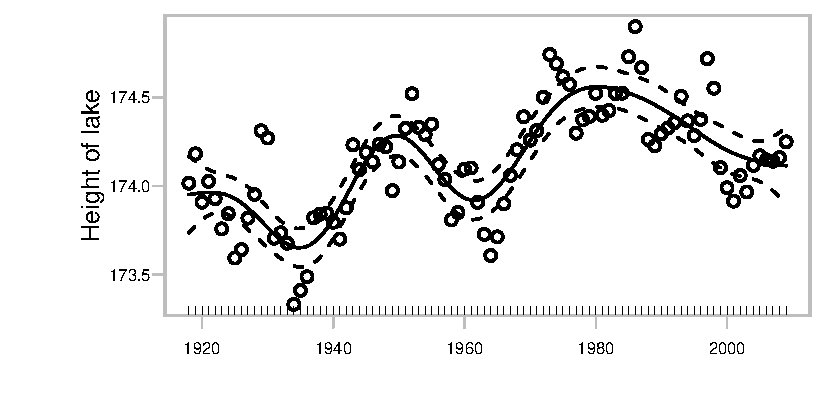
\includegraphics[width=0.98\textwidth]{figs/9-gamErie-1} }

\end{Schunk}
\caption{GAM smoothing term, fitted to the Lake Erie Data.
    Most of the autocorrelation structure has been
    removed, leaving residuals that are very nearly independent.
  }\label{lh-smoothplot}
\end{figure}
%$

\begin{marginfigure}[-3.5cm]
\begin{Schunk}
\begin{Sinput}
## Code
library(mgcv)
df <-  data.frame(
  height=as.vector(Erie),
  year=time(Erie))
obj <- gam(height ~ s(year),
           data=df)
plot(obj, fg="gray",
     shift=mean(df$height),
     residuals=TRUE, pch=1,
     xlab="",
     ylab="Height of lake")
\end{Sinput}
\end{Schunk}
\end{marginfigure}

While smoothing methods that asssume independent errors can be
used, as in Figure \ref{lh-smoothplot}, to fit a curve to such
data, the curve will not be repeatable.  Figure \ref{lh-smoothplot}
does not separate systematic effects from effects due to processes
that evolve in time. Figure \ref{lh-smoothplot} uses the
abilities of the \pkg{mgcv} package, assuming independently and
identically distributed data (hence, no serial correlation!) to
make an automatic choice of the smoothing parameter.  
As the curve is conditional on a particular realization of the process
that generated it, its usefulness is limited.

The pointwise confidence limits are similarly conditioned, relevant
perhaps for interpolalation given this particular realization.
All that is repeatable, given another realization, is the
process that generated the curve, not the curve itself. 

\subsection{Fitting and use of an autoregressive model}

There are several different types of time series models that
may be used to model the correlatios structure, allowing realistic estimates of the lake level a short time ahead, with realistic
confidence bounds around those estimates.  For the Lake Erie
data, an autoregressive correlation structure does a good job of
accounting for the pattern of change around a mean that stays
constant.

Figure \ref{erie-lagplot} suggested that a correlation between each
year and the previous year accounted for the main part of the
autocorrelation structure in Figure \ref{fig:erie}. An AR1 model
(autoregressive with a correlation at lag 1 only), which we now fit,
formalizes this.
\begin{Schunk}
\begin{Sinput}
ar(Erie, order.max=1)
\end{Sinput}
\begin{Soutput}

Call:
ar(x = Erie, order.max = 1)

Coefficients:
    1  
0.851  

Order selected 1  sigma^2 estimated as  0.0291
\end{Soutput}
\end{Schunk}
The one coefficient that is now given is the lag 1 correlation,
equalling 0.851.

\begin{figure}
\begin{Schunk}


\centerline{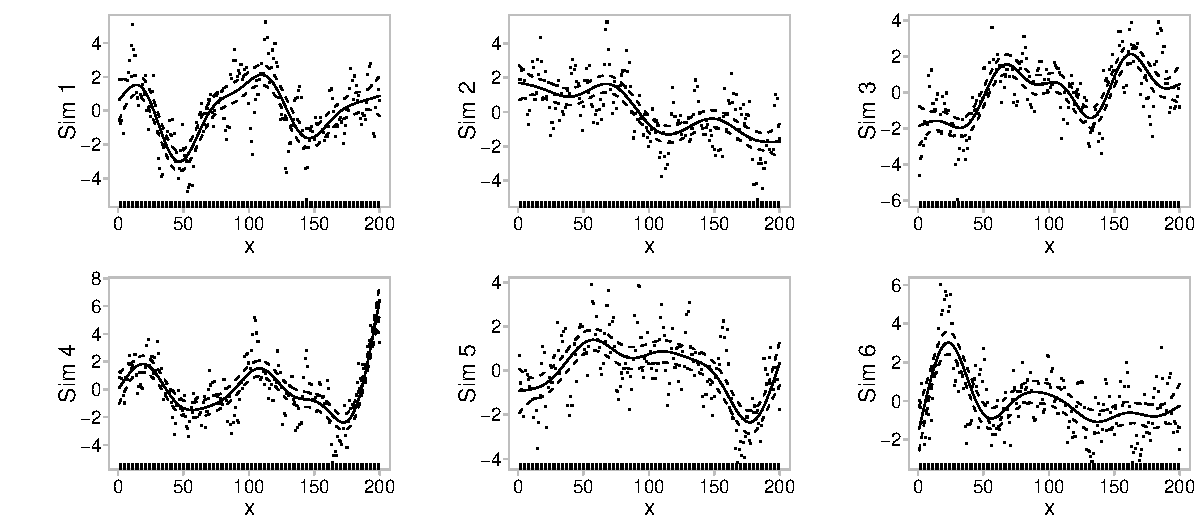
\includegraphics[width=0.97\textwidth]{figs/9-arima-sim-1} }

\end{Schunk}
\caption{The plots are from repeated simulations of an AR1 process
with a lag 1 correlation of 0.85.  Smooth curves, assuming independent
  errors, have been fitted.}\label{fig:ar1fits}
\end{figure}

\begin{marginfigure}[-1.5cm]
\begin{Schunk}
\begin{Sinput}
for (i in 1:6){
ysim <-
  arima.sim(list(ar=0.85),
            n=200)
df <- data.frame(x=1:200,
                 y=ysim)
df.gam <- gam(y ~ s(x),
              data=df)
plot(df.gam, fg="gray",
     ylab=paste("Sim", i),
     residuals=TRUE)
}
\end{Sinput}
\end{Schunk}
\end{marginfigure}

Figure \ref{fig:ar1fits} then investigates how repeated simulations of
this process, with a lag 1 correlation of 0.0.85, compare with Figure
\ref{fig:erie}.  This illustrates the point that a GAM smooth will
extract, from an autoregressive process with mean 0, a pattern that is
not repeatable when the process is re-run.

The curves are different on each occasion.  For generalization beyond
the particular realization that generated them, they serve no useful
purpose.

Once an autoregressive model has been fitted, the function
\code{forecast()} in the \pkg{forecast} package can be used to
predict future levels, albeit with very wide confidence bounds.
For this, it is necessary to refit the model using the function
\code{arima()}. An arima model with order (1,0,0) is an autoregressive
model with order 1.
\vspace*{10pt}

\begin{figure}
\begin{Schunk}


\centerline{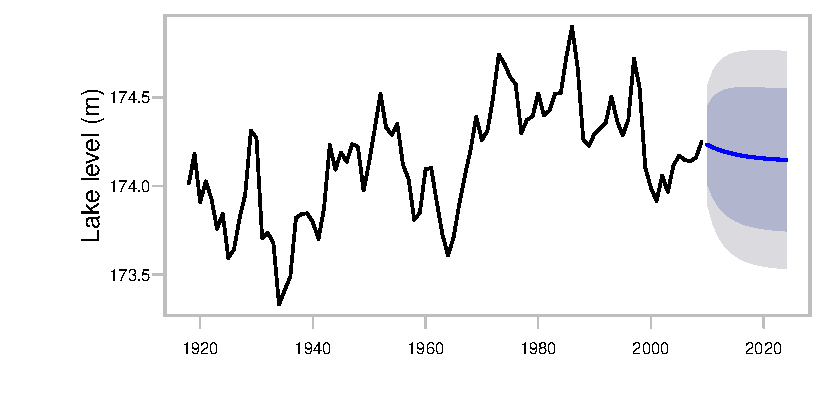
\includegraphics[width=0.98\textwidth]{figs/9-Erie-fcast-1} }

\end{Schunk}
\caption{Predictions, 15 years into the future, of lake levels
  (m). The shaded areas give 80\% and 95\% confidence bounds.
}\label{Erie-fcastplot}
\setfloatalignment{t}
\end{figure}

\begin{marginfigure}[-5cm]
\begin{Schunk}
\begin{Sinput}
erie.ar <- arima(Erie,
            order=c(1,0,0))
library(forecast)
fc <- forecast(erie.ar,
               h=15)
plot(fc, main="", fg="gray",
     ylab="Lake level (m)")
  # 15 time points ahead
\end{Sinput}
\end{Schunk}
\end{marginfigure}

This brief excursion into a simple form of time series model is
intended only to indicate the limitations of automatic smooths.  and
to give a sense of the broad style of time series modeling.  The list
of references at the end of the chapter has details of several books
on time series.

\subsection{Regression with time series errors}

Figure \ref{fig:mdbRainSM} fits annual rainfall, in the Murray-Darling basin of
Australia, as a sum of smooth functions of \code{Year} and \code{SOI}.
Figure \ref{fig:mdbRain} shows the estimated contributions of the two
model terms.
\begin{Schunk}
\begin{Sinput}
## Code
bomregions <- DAAG::bomregions2018
mdbRain.gam <- gam(mdbRain ~ s(Year) + s(SOI),
                   data=bomregions)
plot(mdbRain.gam, residuals=TRUE, se=2, fg="gray",
     pch=1, select=1, cex=1.35, ylab="Partial, Year")
mtext(side=3, line=0.75, "A: Effect of Year", adj=0)
plot(mdbRain.gam, residuals=TRUE, se=2, fg="gray",
     pch=1, select=2, cex=1.35, ylab="Partial, SOI")
mtext(side=3, line=0.75, "B: Effect of SOI", adj=0)
\end{Sinput}
\end{Schunk}
\begin{figure}
\begin{Schunk}


\centerline{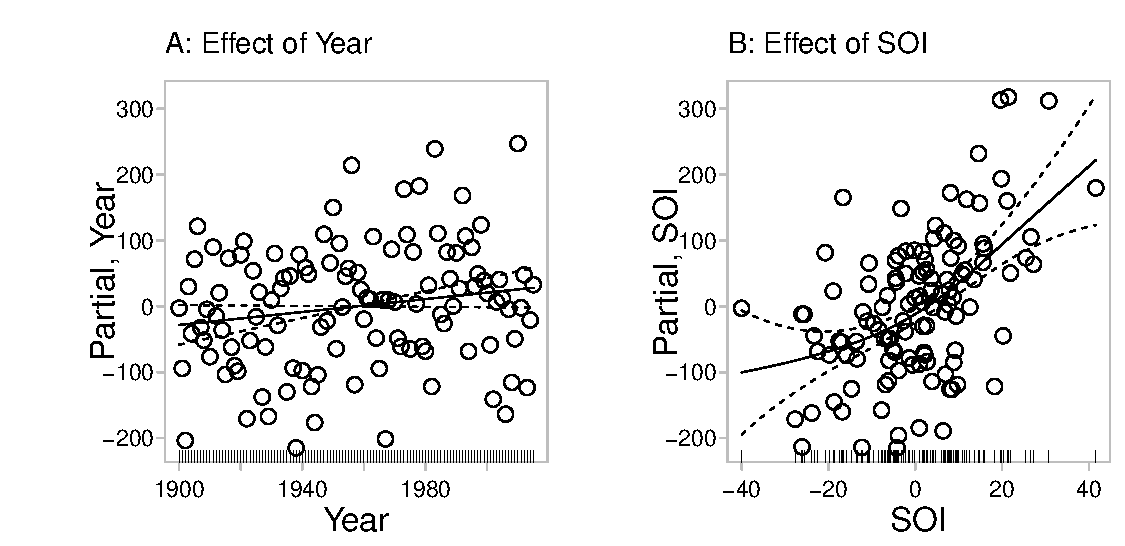
\includegraphics[width=\textwidth]{figs/9-mdb-gam-1} }

\end{Schunk}
  \caption{Estimated contributions of model terms to
    \code{mdbRain}, in a GAM model that adds smooth terms in
    \code{Year} and \code{Rain}. The dashed curves show pointwise
    2-SE limits, for the fitted curve.}\label{fig:mdbRainSM}
\end{figure}

The left panel indicates a consistent pattern of increase of rainfall
with succeeding years, given an adjustment for the effect of SOI.
Errors from the fitted model are consistent with the independent
errors assumption.  The model has then identified a pattern of
increase of rainfall with time, given SOI, that does seem real.  It is
necessary to warn against reliance on extrapolation more than a few
time points into the future. While the result is consistent with
expected effects from global warming, those effects are known to play
out very differently in different parts of the globe.

\subsection*{Investigation of the residual error structure}
Sequential correlation structures are often effective, with
data collected over time, for use in modeling departure from
iid errors.  Where there is such structure structure in the
data, the methodology will if possible use a smooth
curve to account for it.

The residuals can be checked to determine whether the fitted curve
has removed most of the correlation structure in the data.
Figure \ref{fig:ar1sims} shows the autocorrelation function of the
residuals, followed by autocorrelation functions for several series of
independent random normal numbers.  Apart from the weakly attested
correlation at a lag of 12 years, which is a commonplace of weather
data, the pattern of sequential correlation is not much different from
what can be expected in a sequence of independent random normal
numbers.

\begin{figure*}
\begin{Schunk}


\centerline{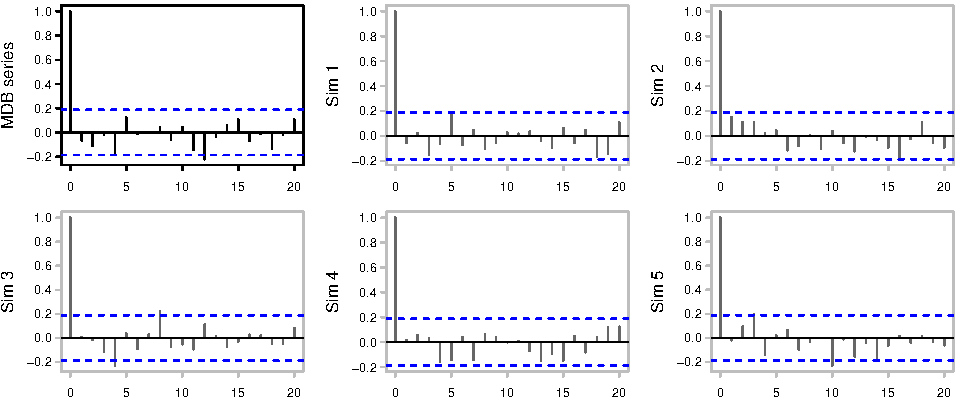
\includegraphics[width=0.97\textwidth]{figs/9-ar1sims-1} }

\end{Schunk}
\caption{The top left panel shows the autocorrelations of the
  residuals from the model \code{mdbRain.gam}.  The five remaining
  panels are the equivalent plots for sequences of independent random
  normal numbers.}\label{fig:ar1sims}
\end{figure*}

Code is:
\begin{Schunk}
\begin{Sinput}
mdbRain.gam <- gam(mdbRain ~ s(Year) + s(SOI),
                   data=bomregions)
n <-  dim(bomregions)[1]
acf(resid(mdbRain.gam), ylab="MDB series")
for(i in 1:5)acf(rnorm(n), ylab=paste("Sim",i),
                 fg="gray", col="gray40")
\end{Sinput}
\end{Schunk}

\subsection{$^*$Box-Jenkins ARIMA Time Series Modeling}

\marginnote{Models that are closely analagous to ARIMA models had
 been used earlier in control theory.  ARIMA models are feedback systems!}
From the perspective of the Box-Jenkins ARIMA (Autoregressive
Integrated Moving Average) approach to time series models,
autoregressive models are a special case.  Many standard types of time
series can be modeled very satisfactorily as ARIMA processes.

\subsection*{Exercise}
The simulations in Figure \ref{fig:ar1fits} show a pattern of
  variation that seems not too different from that in the actual series.
  Modeling of the process as an ARMA or ARIMA process (i.e., allow
  for a moving average term) may do even better.  Use the
  \code{auto.arima()} function in the \pkg{forecast} package to fit an
  ARIMA process:

\subsection{Count Data with Poisson Errors}

\marginnote{Data are a time series.  Serious accidents are
sufficiently uncommon that joint occurrences, or cases
where one event changes the probability of the next,
seem likely to be uncommon.}

Data is for aircraft accidents, from the website
\url{http://www.planecrashinfo.com/}.  The 1920 file has
accidents starting from 1908. The full data are in the
dataset \code{gamclass::airAccs}.
Such issues as there are with sequential correlation
can be ameliorated by working with weekly, rather than daily,
counts. 



\begin{fullwidth}
\begin{figure*}
\vspace*{-12pt}
\begin{Schunk}


\centerline{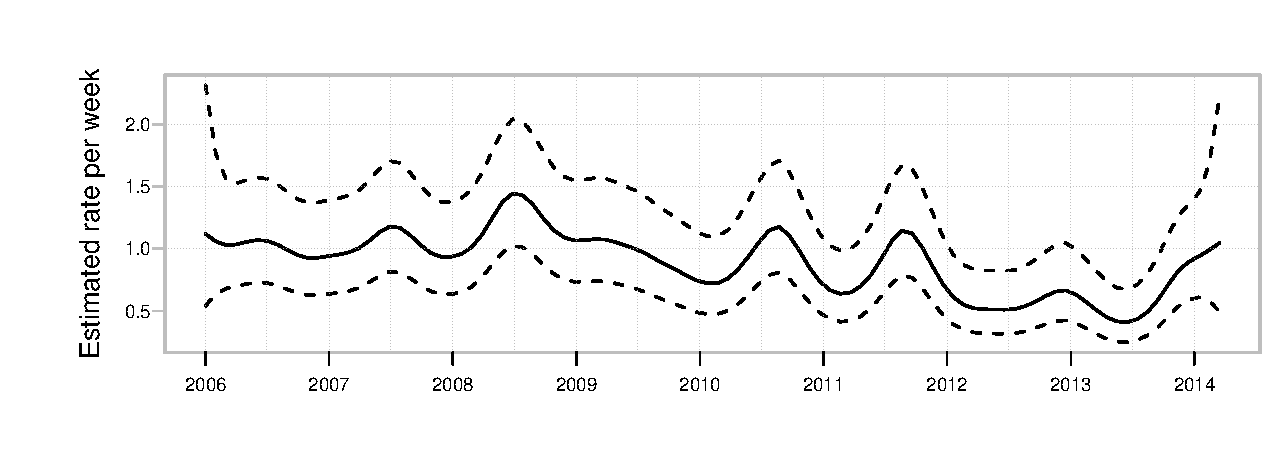
\includegraphics[width=0.98\textwidth]{figs/9-plotGAM-byWk-1} }

\end{Schunk}
\vspace*{-6pt}
\caption{Estimated number of events (aircraft crashes) per week,
  versus time.  The yearly tick marks are for January 1 of the
  stated year.\label{fig:planeCrash}}
\end{figure*}
\end{fullwidth}

Figure \ref{fig:planeCrash} shows a fitted smooth curve, with
pointwise confidence bounds, from a GAM smoothing model that
was fitted to the weekly counts. 

\marginnote[9pt]{See Section \ref{ss:dates} for further details
on the function \code{eventCounts()}.}
\begin{Schunk}
\begin{Sinput}
## Code
airAccs <- gamclass::airAccs
fromDate <- as.Date("2006-01-01")
dfWeek06 <- gamclass::eventCounts(airAccs, dateCol="Date",
                                  from=fromDate,
                                by="1 week", prefix="num")
dfWeek06$day <- julian(dfWeek06$Date, origin=fromDate)
\end{Sinput}
\end{Schunk}
The function \code{gamclass::eventCounts()} was used to create
weekly counts of accidents from January 1, 2006:

Code for Figure \ref{fig:planeCrash} is then.
\begin{fullwidth}

\begin{Schunk}
\begin{Sinput}
## Code
library(mgcv)
year <- seq(from=fromDate, to=max(dfWeek06$Date), by="1 year")
at6 <- julian(seq(from=fromDate, to=max(dfWeek06$Date), by="6 months"), origin=fromDate)
atyear <- julian(year, origin=fromDate)
dfWeek06.gam <- gam(num~s(day, k=200), data=dfWeek06, family=quasipoisson)
avWk <- mean(predict(dfWeek06.gam))
plot(dfWeek06.gam, xaxt="n", shift=avWk, trans=exp, rug=FALSE,
     xlab="", ylab="Estimated rate per week", fg="gray")
axis(1, at=atyear, labels=format(year, "%Y"), lwd=0, lwd.ticks=1)
abline(h=0.5+(1:4)*0.5, v=at6, col="gray", lty=3, lwd=0.5)
\end{Sinput}
\end{Schunk}

\end{fullwidth}

The argument `\code{k}' to the function \code{s()} that sets up the
smooth controls the temporal resolution.  A large \code{k} allows,
if the data seem to justify it, for fine resolution. A penalty is
applied that discriminates against curves that are overly `wiggly'.

Not all count data is suitable for modeling assuming a Poisson type
rare event distribution. For example, the dataset
\url{http://maths-people.anu.edu.au/~johnm/stats-issues/data/hurric2014.csv}
has details, for the years 1950-2012, of US deaths from Atlantic
hurricanes.  For any given hurricane, deaths are not at all independent
rare events.

\section{Classification}

Classification models \marginnote{For the special case $g = 2$,
logistic regression models are an alternative.}
have the character of regression models where
the outcome is categorical, one of $g$ classes.  The
\texttt{fgl} (forensic glass) dataset that will be used as an example
has measurements of each on nine physical properties, for 214 samples
of glass that are classified into $g=6$ different glass types.  

This section will describe a very limited range of available
approaches.  For details
on how and why these methods work, it will be necessary to look
elsewhere.\sidenote{Limited further details and references are provided in \citet{daagur_2011}.}

Linear discriminant analysis (LDA), and quadratic
discriminant analysis (QDA) which slightly generalizes LDA,
both use linear functions of the explanatory variables in the
modeling of the probabilities of group membership.  These
methods will be contrasted with the strongly non-parameteric
approaches of tree-based classification and of random forests.

\subsection*{Linear and quadratic discriminant analysis}

The functions that will be used are \code{lda()}
and \code{qda()}, from the \pkg{MASS} package.  The function
\code{lda()} implements linear discriminant analysis, while
\code{qda()} implements quadratic discriminant analysis.\sidenote{Quadratic
discriminant analysis is an adaptation of linear discriminant analysis
to handle data where the variance-covariance matrices of the different
classes are markedly different.}

\begin{Schunk}
\begin{Sinput}
library(MASS, quietly=TRUE)
\end{Sinput}
\end{Schunk}

Results from use of \code{lda()} lead very
  naturally to useful and informative plots.  Where \code{lda()}
  gives results that are a sub-optimal fit to the data,
  the plots may hint at what type of alternative method
  may be preferable.  They may identify subgroups of
  the orginal $g$ groups, and/or identify points that seem
  misclassified.   

An attractive feature of \code{lda()} is that the discriminant rule
that is obtained has a natural representation $r$-dimensional space.
Providing that there is sufficient independent covariate data, $r$ =
$g-1$.  The analysis leads\sidenote{This is based on a {\em spectral}
  decomposition of the model matrix.}  to $r$ sets of scores, where
each set of scores explains a successively smaller (or at least, not
larger) proportion of the sum of squares of differences of group means
from the overall mean.
\marginnote{With three groups, two dimensions will account for
  all the variation.  A scatterplot is then a geometrically complete
  representation of what the analysis has achieved.}
The $r$ sets of scores can be examined using a
pairs plot.  With larger numbers of groups, it will often happen that
two or at most three dimensions will account for most of the
variation.

\subsection*{Use of \code{lda()} to analyse the forensic glass data}

As noted above, the data frame \code{fgl} has 10 measured physical
characteristics for each of 214 glass fragments that are classified
into 6 different types.  First, fit a linear discriminant analysis,
and use leave-one-out cross-validation to check the accuracy, thus:
\begin{Schunk}
\begin{Sinput}
fglCV.lda <- lda(type ~ ., data=fgl, CV=TRUE)
tab <- table(fgl$type, fglCV.lda$class)
## Confusion matrix
print(round(apply(tab, 1, function(x)x/sum(x)),
            digits=3))
\end{Sinput}
\begin{Soutput}
       
         WinF WinNF   Veh   Con  Tabl  Head
  WinF  0.729 0.237 0.647 0.000 0.111 0.034
  WinNF 0.229 0.684 0.353 0.462 0.222 0.069
  Veh   0.043 0.000 0.000 0.000 0.000 0.000
  Con   0.000 0.039 0.000 0.462 0.000 0.034
  Tabl  0.000 0.026 0.000 0.000 0.556 0.000
  Head  0.000 0.013 0.000 0.077 0.111 0.862
\end{Soutput}
\end{Schunk}

The function \code{confusion()} (\pkg{DAAG}) makes it easy to
get all the above output.  Enter:
\begin{Schunk}
\begin{Sinput}
library(DAAG)
confusion(fgl$type, fglCV.lda$class)
\end{Sinput}
\end{Schunk}

\subsection*{Two-dimensional representation}

Now fit the model with \code{CV=FALSE}, which is the default:
\begin{Schunk}
\begin{Sinput}
fgl.lda <- lda(type ~ ., data=fgl)
\end{Sinput}
\end{Schunk}
The final three lines of the output, obtained by entering
\code{fgl.lda} at the command line, are:
\begin{Schunk}
\begin{Soutput}
Proportion of trace:
  LD1   LD2   LD3   LD4   LD5
0.815 0.117 0.041 0.016 0.011
\end{Soutput}
\end{Schunk}
The numbers \marginnote{Observe that most of the
discriminatory power is in the first two dimensions.}
show the successive proportions of a measure of the
variation that are accounted for by projections onto spaces with
successively larger numbers of dimensions.  

% $

\begin{figure}
\begin{Schunk}


\centerline{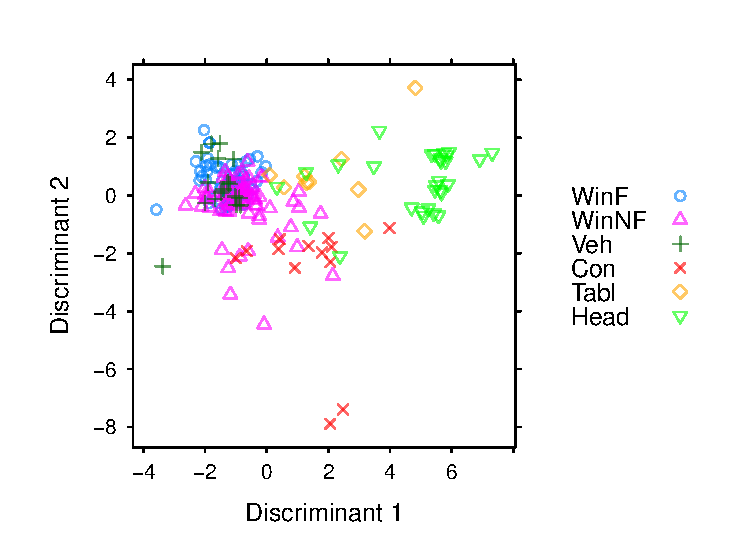
\includegraphics[width=0.9\textwidth]{figs/9-fgl-scores2D-1} }

\end{Schunk}
\caption{Visual representation of scores from a
  {\em linear discriminant analysis}, for the forensic glass data.  A
  six-dimensional pattern of separation between the categories has
  been collapsed to two dimensions.  Some categories may therefore
be better distinguished than is evident from this figure.\label{fig:fgl}}
\end{figure}

Figure \ref{fig:fgl} shows the two-dimensional
representation.
\begin{Schunk}
\begin{Sinput}
library(lattice)
scores <- predict(fgl.lda)$x
xyplot(scores[,2] ~ scores[,1], groups=fgl$type,
       xlab="Discriminant 1",
       ylab="Discriminant 2",
       aspect=1, scales=list(tck=0.4),
       auto.key=list(space="right"),
\end{Sinput}
\end{Schunk}

\marginnote{See Figure \ref{fig:rfbronchit} in Subsection \ref{ss:rf},
for an example of the type of low-dimensional representation that is
possible for results from a randdom forest classification.}
Additionally, it may be useful to examine the plot of the third
versus the second discriminant.  Better still, use the abilites of the
\pkg{rgl} package to examine a 3-dimensional dynamic representation.
With most other methods, a low-dimensional representation does not
arise so directly from the analysis.

\subsection*{Two groups -- comparison with logistic regression}

\marginnote{More technical points, as they apply to the use of
  R's function \code{glm()} for logistic regression, are:
  \begin{itemizz}
\item[-] The fitting procedure minimizes the {\em deviance}. This
  equals 2 ( {\em loglikelihood} for fitted model, minus the
  loglikelihood for the `saturated' model). The `saturated model
  has predicted values equal to observed values.
\item[-] Standard errors and Wald statistics (roughly comparable to
  $t$-statistics) are given for parameter estimates.  These
  depend on approximations that may fail if predicted proportions are
  close to 0 or 1 and/or the sample size is small.
\end{itemizz}
}

The approach is to model the probability of class membership given
the covariates, using the same logistic fixed part of the model as
for linear and quadratic discriminant analysis.  With $\pi$ equal
to the probability of membership in the second class, the model
assumes that
\[ \log(\pi/(1-\pi) = \beta' \mathbf{x}\]
where $\beta$ is a vector of  coefficients that are to be estimated,
and $\mathbf{x}$ is a vector of covariate values.

A logistic regression model is a special case of a Generalized
Linear Model (GLM), as implemented by R's function \code{glm()}. 
There is no provision to adjust predictions to take account of
prior probabilities, though this can be done as an add-on to the analysis.
Other points of difference from linear discriminant analysis are:

\begin{itemize}
\item Inference is conditional on the observed covariate values. A model
  for the probability of covariate values $\mathbf{x}$ given the class
  $c$, as for linear discriminant analysis, is not required.
  (Linear discriminant analysis assumes a multivariate normal distribution
  assumptions for $\mathbf{x}$, given the class $c$. In practice, results
  seem relatively robust against failure of this assumption.)
\item The logit model uses the {\em link} function $f(\pi) =
  \log(\pi/(1-\pi)$. Other choices of link function are available.
  Where there are sufficient data to check whether one of these other
  links may be more appropriate, this should be checked.  Or there may
  be previous experience with comparable data that suggests use of a
  link other than the logit.
\item Observations can be given prior weights.
\end{itemize}

\section{Tree-based methods and random forests}
On a scale in which highly parametric methods lie at one end and
highly non-parametric methods at the other, linear discriminant
methods lie at the parametric end, and tree-based methods and random
forests at the non-parametric extreme.  An attraction of tree-based
methods and random forests is that model choice can be pretty much
automated.

We begin by loading the \pkg{rpart} package:
\begin{Schunk}
\begin{Sinput}
library(rpart)
\end{Sinput}
\end{Schunk}

\marginnote[12pt]{The dataset \margtt{bronchit} may alternatively be
found in the \pkg{SMIR} package.}
For the calculations that follow, data are columns in the data frame
\texttt{bronchit}, in the \pkg{DAAGviz} package.
\marginnote[12pt]{Here \margtt{r=1} denotes bronchitis,  while \code{r=0}
indicates that bronchitis is absent.}
\begin{Schunk}
\begin{Sinput}
bronchit <- DAAGviz::bronchit
head(bronchit, 3)
\end{Sinput}
\begin{Soutput}
  r  cig poll
1 0 5.15 67.1
2 0 6.75 64.4
3 0 0.00 65.9
\end{Soutput}
\end{Schunk}
In place of the variable \code{r} with values 0 and 1, we use a
factor with levels \code{abs} and \code{pres}. Labels that appear
in the output are then more meaningful.
\begin{Schunk}
\begin{Sinput}
## Now make the outcome variable a factor
bronchit <-
  within(bronchit,
         rfac <- factor(r, labels=c("abs","pres")))
\end{Sinput}
\end{Schunk}

\marginnote[12pt]{With a factor (\code{rfac}) as outcome,
\margtt{method="class"} is the default. Setting
\margtt{method="class"}, to make it quite clear that
we are using a splitting rule that is appropriate to
a categorical (rather than continuous) outcome, is good
practice.}
The following fits a tree-based model:
\begin{Schunk}
\begin{Sinput}
set.seed(47)   # Reproduce tree shown
b.rpart <- rpart(rfac ~ cig+poll, data=bronchit,
                 method="class")
\end{Sinput}
\end{Schunk}

The `complexity' paremeter \code{cp}, by default set to 0.01,
controls how far splitting continues.  In practice, it is usual to
set \code{cp} small enough that splitting continues further than
is optimal, then pruning the tree back. Cross-validation based
accuracies are calculated at each split, and can be used to determine
the optimal depth of tree.  Details will not be given at this point,
as the interest is in trees as a lead-in to random forests.  For
random forests, the depth of the splits in individual trees is not
of great consequence --- it is not important for individual trees
to be optimal.

Figure \ref{fig:tree} is a visual summary of results from the
tree-based classification, designed to predict the probability that a
miner will have bronchitis.  Where the condition at a node is
satisfied, the left branch is taken. Thus, at the initial node,
\code{cig$<$4.385} takes the branch to the left.  In general (no
random number seed), the tree may be different for each
different run of the calculations.

\begin{marginfigure}
\begin{Schunk}


\centerline{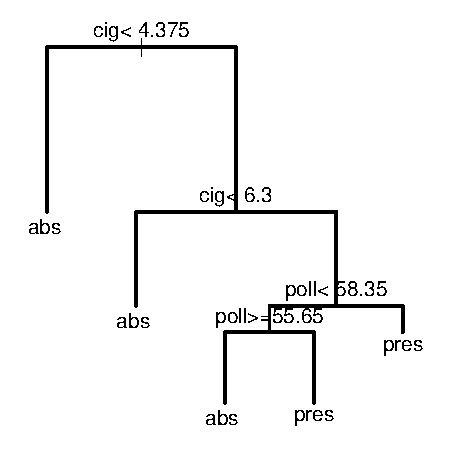
\includegraphics[width=0.98\textwidth]{figs/9-treefig-1} }

\end{Schunk}
\caption{Decision tree for predicting whether a miner has
    bronchitis.
}\label{fig:tree}
\end{marginfigure} 

Tree-based classification proceeds by constructing a sequence of
decision steps. At each node, the split is used that best separates
the data into two groups.  Here (Figure \ref{fig:tree}) tree-based
regression does unusually well (CV accuracy = 97.2\%), perhaps because
it is well designed to reproduce a simple form of sequential decision
rule that has been used by the clinicians.

\begin{marginfigure}
Code for Figure \ref{fig:tree} is:
\begin{Schunk}
\begin{Sinput}
plot(b.rpart)
text(b.rpart, xpd=TRUE)
\end{Sinput}
\end{Schunk}
\end{marginfigure}

How is `best' defined? Splits are chosen so that the Gini index of
`impurity' is minimized.  Other criteria are possible, but this is
how \code{randomForest()} constructs its trees.

\subsection{Random forests}\label{ss:rf}

\begin{Schunk}
\begin{Sinput}
library(randomForest, quietly=TRUE)
\end{Sinput}
\end{Schunk}

Figure \ref{fig:brontrees} shows trees that have been fitted to
different bootstrap samples of the bronchitis data.  Typically 500 or
more trees are fitted, without a stopping rule.  Individual trees are
likely to overfit.  As each tree is for a different random sample of
the data, there is no overfitting overall.

\begin{figure}
\begin{Schunk}


\centerline{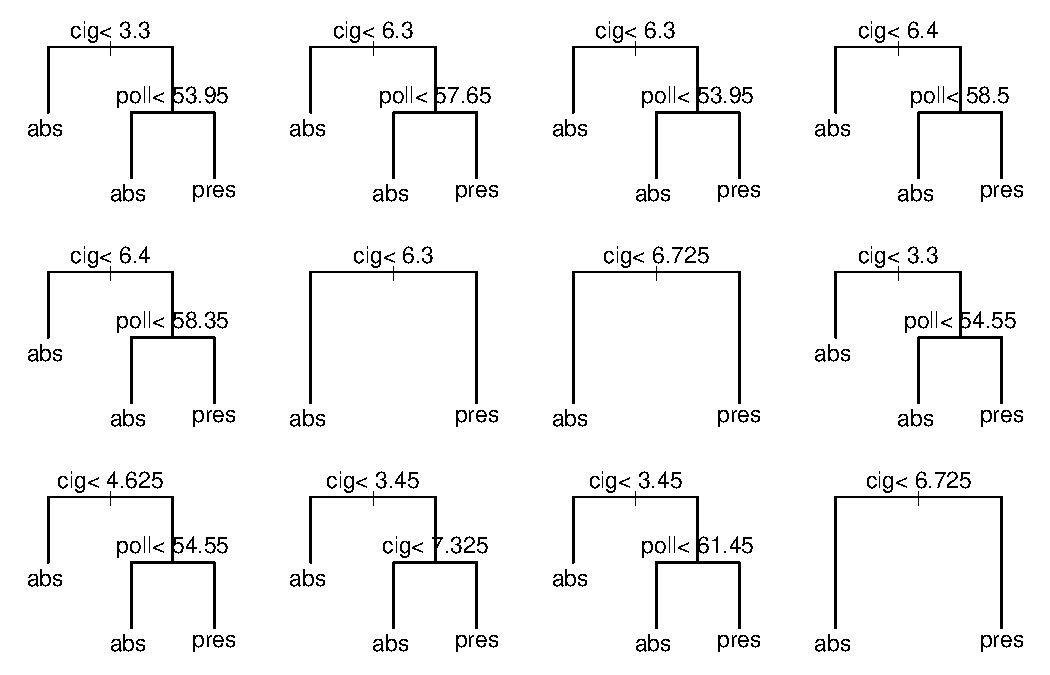
\includegraphics[width=0.85\textwidth]{figs/9-rf-x-bronchit-1} }

\end{Schunk}
\caption{Each tree is for a different bootstrap sample of
  observations.  The final classification is determined by a random
  vote over all trees.  Where there are $>$ 2 explanatory variables
  (but not here) a different random sample of variables is typically
  used for each different split. The final classification is
  determined by a random vote over all trees.}\label{fig:brontrees}
\end{figure}

For each bootstrap sample, predictions are made for the observations
that were not included -- i.e., for the out-of-bag data.  Comparison
with the actual group assignments then provides an unbiased estimate
of accuracy.

For the \texttt{bronchit} data, here is the \texttt{randomForest()}
result.
\begin{Schunk}
\begin{Sinput}
(bronchit.rf <- randomForest(rfac ~ cig+poll,
                             data=bronchit))
\end{Sinput}
\begin{Soutput}

Call:
 randomForest(formula = rfac ~ cig + poll, data = bronchit) 
               Type of random forest: classification
                     Number of trees: 500
No. of variables tried at each split: 1

        OOB estimate of  error rate: 23.58%
Confusion matrix:
     abs pres class.error
abs  145   21      0.1265
pres  29   17      0.6304
\end{Soutput}
\end{Schunk}
The accuracy is much better than the \texttt{rpart()} accuracy.  The
random forest methodology will often improve, sometimes quite
dramatically, on tree-based classification.

\begin{marginfigure}
\begin{Schunk}


\centerline{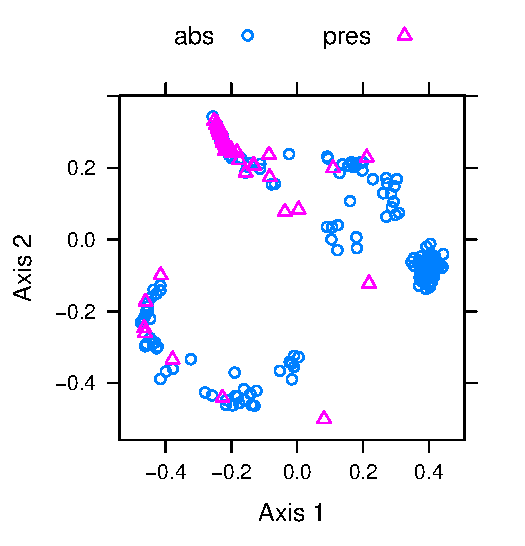
\includegraphics[width=0.98\textwidth]{figs/9-proximity-plot-1} }

\end{Schunk}
\caption{The plot is designed to represent, in two dimensions, the random
  forest result. It aims to reflect probabilities of group membership
  given by the analysis.  It is not derived by a 'scaling' of the
  feature space.
}\label{fig:rfbronchit}
\end{marginfigure}
%$

Figure \ref{fig:rfbronchit} is a visual summary of the random forest
classification result.  The proportion of trees in which any pair of
points appear together at the same node may be used as a measure of
the `proximity' between that pair of points.  Then, subtracting
proximity from one to obtain a measure of distance, an ordination
method is used to find an approximates representation of those points in a
low-dimensional space.

There is a tuning parameter \code{mtry} which controls the number of
randomly chosen variables considered for each tree.  This is not too
much of an issue for the present data, where there are only two
explanatory variables.

Code for Figure \ref{fig:rfbronchit} is:
\begin{Schunk}
\begin{Sinput}
parset <- simpleTheme(pch=1:2)
bronchit.rf <- randomForest(rfac ~ cig+poll,
                            proximity=TRUE,
                            data=bronchit)
points <- cmdscale(1-bronchit.rf$proximity)
xyplot(points[,2] ~ points[,1],
       groups=bronchit$rfac,
       xlab="Axis 1", ylab="Axis 2",
       par.settings=parset, aspect=1,
       auto.key=list(columns=2))
\end{Sinput}
\end{Schunk}

\subsection*{A random forest fit to the forensic glass data}

The algorithm can be used in a highly automatic manner.  Here then is
the random forest analysis for the forensic glass data, leaving the
tuning parameter (\code{mtry}) at its default\sidenote{The default is
  to set \margtt{mtry} to the square root of the total number of
  variables, rounded up to an integral value.}:
\begin{Schunk}
\begin{Sinput}
(fgl.rf <- randomForest(type ~ ., data=fgl))
\end{Sinput}
\begin{Soutput}

Call:
 randomForest(formula = type ~ ., data = fgl) 
               Type of random forest: classification
                     Number of trees: 500
No. of variables tried at each split: 3

        OOB estimate of  error rate: 20.56%
Confusion matrix:
      WinF WinNF Veh Con Tabl Head class.error
WinF    63     6   1   0    0    0      0.1000
WinNF   10    59   1   3    2    1      0.2237
Veh      8     3   6   0    0    0      0.6471
Con      0     3   0   9    0    1      0.3077
Tabl     0     2   0   0    7    0      0.2222
Head     1     2   0   0    0   26      0.1034
\end{Soutput}
\end{Schunk}
This improves substantially on the linear discriminant result.
This may happen because the explanatory variables have effects
that are non-linear on a logit scale.  The more likely reason
is that there are interaction effects, perhaps of a relatively
complicated kind, for which the \code{lda()} analysis has not
accounted.

The predictive accuracy might be further improved by varying the
tuning parameter \code{mtry} from its default.  See \code{help(tuneRF)}
for details of the function \code{tuneRF()} that is designed to
assist in finding the optimum choice of \code{mtry}.

\section{$^*$Ordination}

Ordination is a generic name for methods for providing a low-dimensional
view of points in multi-dimensional space, such that `similar' objects
are near each other and dissimilar objects are separated.  The plot(s)
from an ordination in 2 or 3 dimensions may provide useful visual clues
on clusters in the data and/or on outliers.

The ordination methods described here are all versions of
multi-dimensional scaling (MDS).  If distances are not already given,
a first task is to calculate `distances' between points.  Or if
similarities are given, they must be first be transformed into 
`distances'.

From Australian road travel distances 
\marginnote{An ordination might alternatively be based on road travel
  times, or on air travel times.}
between cities and larger towns,
can we derive a plausible `map', or `ordination', showing the relative
locations?  The resulting `map' would give a better indication
than a geographical map of the road travel effort involved in getting
from one place to another.

Genomic data provides another example. Various methods are available
for calculating genomic `distances' between, e.g., different insect
species. The distance measures are based on evolutionary models that
aim to give distances between pairs of species that are a monotone
function of the time since the two species separated.

One standard type of problem starts from a matrix $\bX$ of $n$
observations by $p$ variables, then seeking a low-dimensional
representation.  A first step is then to calculate distances between
observations.\sidenote{Principal components analysis
  circumvents the calculation of distances, for the commonly used
  Euclidean distance measure.  See below.}
  The hope is that a major part of the information
content in the $p$ variables, as it relates to the separation between
observations, can be pretty much summarized in a small number of
constructed variables.

There is typically no good model, equivalent
to the evolutionary models used by molecular biologists, that can be
used to motivate distance calculations.  There is then a large element
of arbritariness in the distance measure used.
Results may depend strongly on the distance measure used.  Unless
measurements are comparable (e.g., relative growth, as measured
perhaps on a logarithmic scale, for different body measurements), it
is usually desirable to calculate distances from standardized variable
values.  This is done by subtracting the mean and dividing by the
standard deviation.

If data can be separated into known classes that should be reflected
in any ordination, then the scores from classification using
\code{lda()} may be a good basis for an ordination. Plots in 2 or
perhaps 3 dimensions may then reveal additional classes and/or
identify points that may be misclassified and/or are in some sense
outliers.  They give an indication of the effectiveness of the
discrimination method in choosing the boundaries between classes.

Figure \ref{fig:rfbronchit} demonstrated the use of `proximities'
that are available from \code{randomForest()} as measures of the
closeness of any pair of points.  These were then turned into rough
distance measures that then formed the basis for an ordination.  With
Support Vector Machines, distance measures can be derived from the
'decision values' and used for ordination.

\subsection{Distance measures}

\subsection*{Euclidean distances}

Treating the rows of $\bX$ ($n$ by $p$) as points in a $p$-dimensional
space, the squared Euclidean distance  $d_{ij}^2$ between points $i$ and $j$ is
\[
 d_{ij}^2 = \sum_{k=1}^p (x_{ik}-x_{jk})^2
\]
The distances satisfy the triangle inequality\sidenote{This says
  that a straight line is the shortest distance between two points!}
\[ d_{ij} \le d_{ik} + d_{kj} \]

The columns may be weighted differently.\sidenote{More generally, they
  can be arbitrarily transformed before calculating the $d_{ij}$.}
Use of an unweighted measure with all columns scaled to a standard
deviation of one is equivalent to working with the unscaled columns
and calculating $d_{ij}^2$ as
\[
d_{ij}^2 = \sum_{k=1}^p w_{ij} (x_{ik}-x_{jk})^2
\]
where $w_{ij} = (s_i s_j)^{-1}$ is the inverse of the product of
the standard deviations for columns $i$ and $j$.

Where all elements of a column are positive, use of the
logarithmic transformation is common. A logarithmic scale makes sense
for biological morphometric data, and for other data with similar
characteristics.  For morphometric data, the effect is to focus
attention on relative changes in the various body proportions,
rather than on absolute magnitudes.

\subsection*{Non-Euclidean distance measures}

Euclidean distance is one of many possible choices of distance
measures, still satisfying the triangle inequality.  As an example of
a non-Euclidean measure, consider the Manhattan distance.
\marginnote{For the Manhattan distance:
\[
 d_{ij} = \sum_{k=1}^p \mid x_{ik}-x_{jk} \mid
\]
}
The Manhattan distance is the shortest distance for a journey that
always proceeds along one of the co-ordinate axes.  In Manhattan in
New York, streets are laid out in a rectangular grid.  This is then
(with $k=2$) the walking distance along one or other street.  For
other choices, see the help page for the function
\code{dist()}.\sidenote{The function \code{daisy()} in the
  \pkg{cluster} package offers a wider choice, including
  distance measures for factor or ordinal data.  Its
  argument \code{stand} causes prior standardization of data.
\vspace{12pt}
}

\subsection*{From distances to a representation in Euclidean space}

Irrespective of the method of calculation of the distance measure,
ordination methods yield a representation in Euclidean space.  It is
always possible to find a configuration $\sfX$ in Euclidean space in
which the `distances' are approximated, perhaps rather
poorly.\sidenote{This is true whether ot not the triangle inequality
  is satisfied.}  It will become apparent in the course of seeking the
configuration whether an exact embedding (matrix $\sfX$) is possible,
and how accurate this embedding is.
The representation is not
unique.  The matrices $\sfX$ and $\sfX \bP$, where $\bP$ is an
orthonormal matrix, give exactly the same distances.


\subsection*{The connection with principal components}
\marginnote{We assume that none of the columns can be written as a
  linear combination of other columns.}
Let $\bX$ be an $n$ by $p$ matrix that is used for the calculation of
Euclidean distances, after any transformations and/or weighting.
Then metric $p$-dimensional ordination, applied to Euclidean distances
between the rows of $\bX$, yields a representation in $p$-dimensional
space that is formally equivalent to that derived from the use of
principal components.  The function \code{cmdscale()} yields, by a
different set of matrix manipulations, what is essentially a principal
components decomposition.  Principal components circumvents the
calculation of distances.

\subsection*{Semi-metric and non-metric scaling}

\marginnote[12pt]{The assumption of a Euclidean distance scale is a
  convenient starting point for calculations.  An ordination that
  preserves relative rather than absolute distances can often be more
  appropriate.  Additionally, small distances may be measured more
  accurately than large distances.}
Semi-metric and non-metric methods all start from `distances', but
allow greater flexibility in their use to create an ordination. The
aim is to represent the `distances' in some specified number of
dimensions, typically two dimensions.  As described here, a first step
is to treat the distances as Euclidean, and determine a configuration
in Euclidean space.  These Euclidean distances are then used as a
starting point for a representation in which the requirement that
these are Euclidean distances, all determined with equal accuracy, is
relaxed.  The methods that will be noted here are Sammon scaling and
Kruskal's non-metric multidimensional scaling.

\subsection*{Example -- Australian road distances}
The distance matrix that will be used is in the matrix 
\code{DAAG::audists}.  Figure \ref{fig:audists} is from the
use of classical multi-dimensional scaling, as implemented in the
function \code{cmdscale()}:

\noindent
An alternative way to add names of cities or other labels is to use
\code{identify()} to add labels interactively, thus:


\begin{marginfigure}
\begin{Schunk}


\centerline{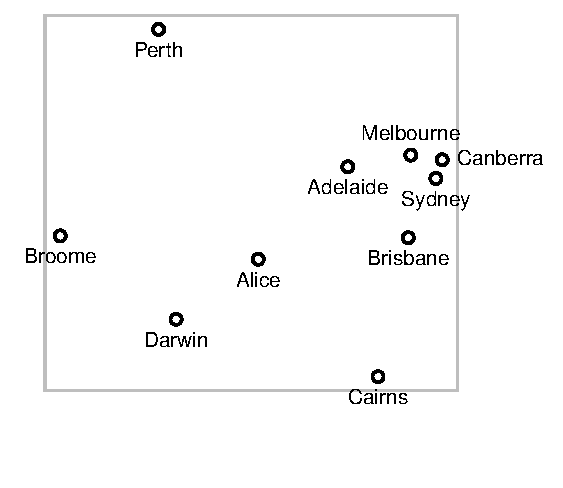
\includegraphics[width=0.98\textwidth]{figs/9-aupoints-1} }

\end{Schunk}
\caption{Relative locations of Australian cities, derived from road
  map distances, using metric scaling.\label{fig:audists}}
\end{marginfigure}
Code is:
\begin{Schunk}
\begin{Sinput}
audists <- DAAG::audists
aupts <- cmdscale(audists)
plot(aupts, axes=FALSE, ann=FALSE, fg="gray",
     frame.plot=TRUE)
city <- rownames(aupts)
pos <- rep(1,length(city))
pos[city=="Melbourne"]<- 3
pos[city=="Canberra"] <- 4
par(xpd=TRUE)
text(aupts, labels=city, pos=pos)
par(xpd=FALSE)
\end{Sinput}
\end{Schunk}


Classical multi-dimensional scaling, as implemented by
 \code{cmdscale()}, gives long distances the same weight as short
 distances.  It is just as prepared to shift Canberra around relative
 to Melbourne and Sydney, as to move Perth.  It makes more sense to
 give reduced weight to long distances, as is done by \code{sammon()}
 (\pkg{MASS}).



\begin{figure*}[h]
\begin{Schunk}


\centerline{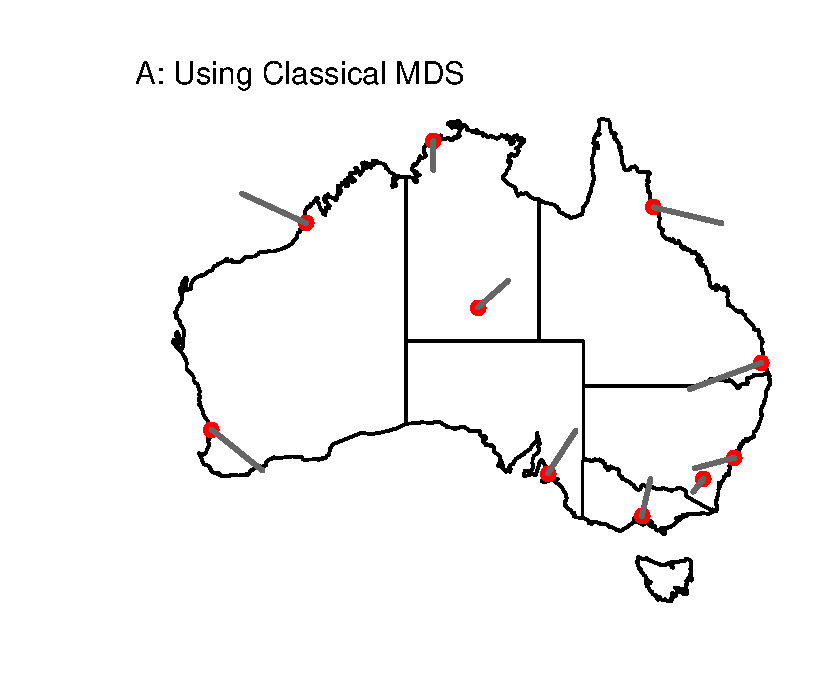
\includegraphics[width=0.47\textwidth]{figs/9-au-both-1} 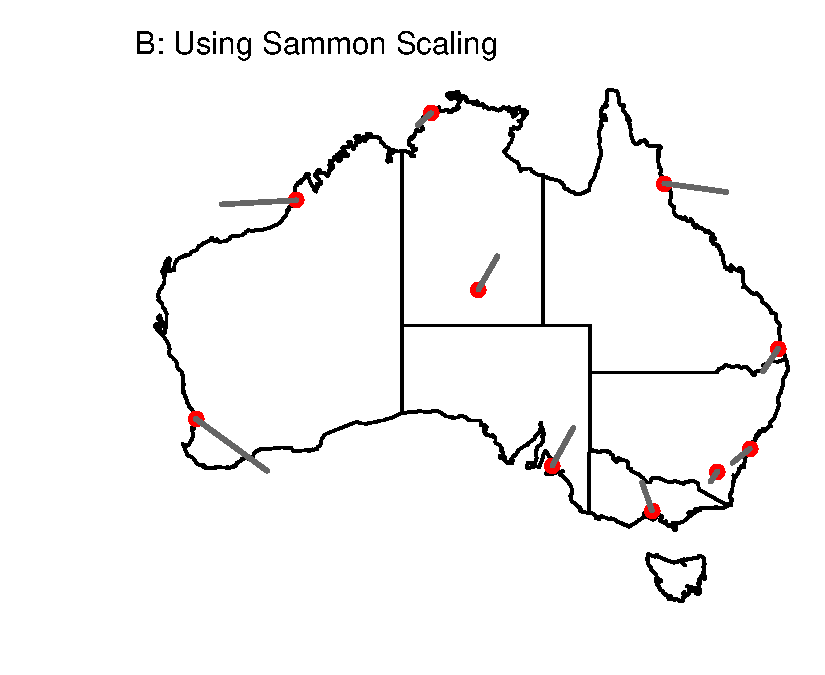
\includegraphics[width=0.47\textwidth]{figs/9-au-both-2} }

\end{Schunk}
      \caption{In Panel A, Figure \ref{fig:audists} has been linearly
        transformed, to give a best fit to a map of Australia.  Each city
        moves as shown by the line that radiates out from it.  Panel B
        is the equivalent plot for Sammon scaling.
\label{fig:aufit}}
 \end{figure*}
 Figure \ref{fig:aufit} shows side by side the overlays of the
 `maps' that result from the different ordinations, onto a physical
 map of Australia.  Panel A shows the result for classical
 multi-dimensional scaling.  Panel B does the same, now for the
 result from Sammon scaling.  Notice how Brisbane, Sydney, Canberra
 and Melbourne now maintain their relative positions better.

The function \code{oz::oz()}, with default arguments, draws an
outline of the coast of Australia, with state boundaries shown.
Arguments are available that can be used to limit what is shown 
(e.g. the NSW and Victorian states only).
To see the code for the overlays onto the map of the Australian
coast, source the file that has the code for the figures of this
chapter, and type:
\begin{Schunk}
\begin{Sinput}
fig9.15A
fig9.15B
\end{Sinput}
\end{Schunk}

The exercise can be repeated for multidimensional scaling (MDS). MDS
preserves only, as far as possible, the relative distances.  A
starting configuration of points is required.  This might come from
the configuration given by \code{cmdscale()}.  For the supplementary
figure \code{supp9.1()} that shows the MDS configuration, however, we
use the physical latitudes and longitudes.

To show this figure, source the file, if this has not been done
previously, that has the code for the figures of this chapter. Then
type:
\begin{Schunk}
\begin{Sinput}
supp9.1()
\end{Sinput}
\end{Schunk}

\section{Maps, map overlays, and spatial analysis}

Extensive information is available both in vignettes included
with R package, and on online.  Code that is provided with
the vignettes can be used to recreate the maps.

\begin{itemizz}
\item[] Lovelace et al.(2014) is a tutorial overview.
\item[] The {\em mapmisc} vignette "Overview of mapping with mapmisc"
shows a number of maps that illustrate some of the possibilities.
\item[] Helpful sources of information on the relevant R data structures
are the \pkg{sf} vignette "Simple Features for R" and the \pkg{tmap} 
vignette "tmap in a nutshell."
\item[] Detailed information on relevant R packages and abilities
is available under \underline{Spatial} on the R Task Views web page
  (\url{https://cran.r-project.org/web/views/Spatial.html}).
  \item[] See articles in the {\em Journal of Statistical Software}
  special volume {\em https://www.jstatsoft.org/issue/view/v063}
  (Volume 6e3, 2015.)
\end{itemizz}

\section*{References}
\begin{itemizz}
\item[] \Citealt{CowpertwaitMet}.
\newblock {\em Introductory Time Series with R.} Springer.
\item[] \Citealt{Hyndman-exp}.
\newblock {\em Forecasting with Exponential Smoothing: The State Space
  Approach.\/} 2$^{nd}$ edn.
\item[] \Citealt{lovelave_cheshire_2014}. \newblock Introduction to visualising spatial data in R. National Centre for Research
Methods Working Papers, 14(03). Retrieved from \url{https://github.com/Robinlovelace/Creating-maps-in-R}.
\item[] \Citealt{taleb_2004}.  \newblock {\em
    Fooled By Randomness: The Hidden Role Of Chance In Life And In The
    Markets.} Random House, 2ed.\newline [Has insightful comments
  on the over-interpretation of phenomena in which randomness is
  likely to have a large role.]
\end{itemizz}
